% Topic #1 - Introduction

%------------------------------------
% Main Settings
%------------------------------------
\documentclass[10pt]{beamer}

%--------------------------------------%
% Set font, and frame title info    %
%--------------------------------------%
\usefonttheme{serif}
\setbeamerfont{frametitle}{series=\bfseries}
\setbeamerfont{framesubtitle}{series=\bfseries}

%--------------------------------------
% "Sub-settings"
%--------------------------------------
\setbeamertemplate{navigation symbols}{}		% Get rid of navigation symbols
\setbeamertemplate{items}[default]				% Uses triangles and numbers instead of 3D balls (which I don't like)
\setbeamertemplate{itemize items}[circle]		% Use circles instead of triangles for itemized lists

%-------------------------------------
% Custom Commands
%-------------------------------------
\newtheorem{hypothesis}{Hypothesis}

%---For Footnotes---%
\usepackage{tikz}
\usetikzlibrary{positioning,calc} % Needed to make angle connector arrows.
\usepackage[absolute,overlay]{textpos}
\newenvironment{reference}[2]{%
	\begin{textblock*}{\textwidth}(#1,#2)
		\tiny\bgroup\color{gray}}{\egroup\end{textblock*}}
%------%		

%----------------------------------------%
% For making definitions in boxes        %
%----------------------------------------%
\usepackage{tcolorbox}

%-- Packages for making nice tables --%
\usepackage{booktabs}
\usepackage{makecell}  % Required for specifying multiple rows within a table cell

%--------------------------------%
%     Custom Colours             %
%--------------------------------%
\usepackage{xcolor}
\definecolor{myblue}{rgb}{0,0.3,0.6}
\definecolor{myblue2}{rgb}{0,0.4,0.8}
\setbeamercolor{frametitle}{fg=myblue}
\setbeamercolor{framesubtitle}{fg=myblue2}
\setbeamercolor{itemize item}{fg=myblue}
\setbeamercolor{itemize subitem}{fg=myblue2}
\setbeamercolor{enumerate item}{fg=myblue}
\setbeamercolor{enumerate subitem}{fg=myblue2}


%----------------------------------%
% Creating nice blocks             %
%----------------------------------%
\setbeamercolor{block title}{bg=myblue, fg=white} %bg=background, fg=foreground
\setbeamercolor{block body}{bg=myblue!20, fg=black} %bg=background, fg=foreground
\setbeamerfont*{block title}{family=\sffamily, series=\bfseries, size=\large}
\setbeamertemplate{blocks}[rounded][shadow=true]

%------------------------------------------
%  Begin Presentations
%------------------------------------------
\begin{document}


%-----------------------%
%  Title Slide          %
%-----------------------%
\begin{frame}
	\begin{tikzpicture}[remember picture,overlay]
		\fill[color=myblue, draw=none] (current page.west) rectangle(current page.north east);
		\node at (1.6, 1.0) {\color{white}\LARGE{\textbf{BIOL 1201:}}};
		\node at (4, 0.2) {\color{white}\LARGE{\textbf{Molecular and Cell Biology}}};
		\node at (0.82, -1.2) {\color{black}\normalsize{Tim Frasier}};
		\node at (1.8, -1.65) {\color{black}{\emph{Saint Mary's University}}};
	\end{tikzpicture}
\end{frame}


%-----------------------%
%     Welcome           %
%-----------------------%
\begin{frame}[t]
\frametitle{Welcome!}

	\vspace{0.5cm}

	\begin{columns}[T]
		\begin{column}{0.5\textwidth}
			\begin{center}
				To SMU\\
				\vspace{0.25cm}
				\includegraphics[width=0.8\textwidth]{figures/smu.jpg}
			\end{center}
		\end{column}
		
		\begin{column}{0.5\textwidth}
			\begin{center}
				To Biology\\
				\vspace{0.25cm}
				\includegraphics[width=1.0\textwidth]{figures/biology.jpg}
			\end{center}
		\end{column}
	\end{columns}	
\end{frame}


%------------------------%
%    Introductions       %
%------------------------%
\begin{frame}[t]
\frametitle{Introductions}
\vspace{0.5cm}
	
	\begin{center}
		\textbf{Dr. Tim Frasier}
	\end{center}
	
	\vspace{0.25cm}
	
	\begin{columns}
		\begin{column}{0.33\textwidth}
			\begin{center}
				\includegraphics[width=1.0\textwidth]{figures/forensics.jpg}
			\end{center}
		\end{column}
		
		\begin{column}{0.33\textwidth}
			\begin{center}
				\includegraphics[width=1.0\textwidth]{figures/pulled.png}
			\end{center}
		\end{column}
		
		\begin{column}{0.33\textwidth}
			\begin{center}
				\includegraphics[width=1.0\textwidth]{figures/biology2.jpg}
			\end{center}
		\end{column}
	\end{columns}
\end{frame}


%--------------------------%
%    Research              %
%--------------------------%
\begin{frame}[t]
\frametitle{Research}

	\begin{center}
		Conservation genetics of endangered whale species
	\end{center}

	\begin{columns}[t]
		\begin{column}{0.5\textwidth}
			\begin{center}
				\includegraphics[width=0.8\textwidth]{figures/rightwhale.jpg}\\
				\vspace{0.25cm}
				\includegraphics[width=0.8\textwidth]{figures/beluga.jpg}
			\end{center}
		\end{column}
		
		\begin{column}{0.5\textwidth}
			\begin{center}
				\includegraphics[width=0.7\textwidth]{figures/orca.jpg}\\
				\vspace{0.25cm}
				\includegraphics[width=0.7\textwidth]{figures/humpback.jpg}
			\end{center}
		\end{column}	
	\end{columns}	
\end{frame}


%---------------------------%
%   Forensics               %
%---------------------------%
\begin{frame}[t]
\frametitle{Forensics}
\vspace{0.25cm}

	\begin{center}
		\includegraphics[width=0.6\textwidth]{figures/nrdpfc.png}\\
		\vspace{0.5cm}
		\includegraphics[width=0.6\textwidth]{figures/rcmp.png}
	\end{center}
\end{frame}


%-----------------------%
%  Cycling              %
%-----------------------%
\begin{frame}
	\begin{columns}
		\begin{column}{0.6\textwidth}
			\begin{center}
				\includegraphics[width=0.75\textwidth]{figures/mamil.png}
			\end{center}
		\end{column}
		
		\begin{column}{0.4\textwidth}
			\includegraphics[width=0.9\textwidth]{figures/cycling1.png}\\
			\vspace{0.5cm}
			\includegraphics[width=0.9\textwidth]{figures/cycling2.png}\\
		\end{column}
	\end{columns}
\end{frame}


%-----------------------%
%  Contact Information  %
%-----------------------%
\begin{frame}[t]
\frametitle{Contact Information}
\vspace{0.5cm}

	\begin{tabular}{@{} l l}
		\textbf{Office:} & Science Building, room S 327\\
		\addlinespace
		\addlinespace
		\textbf{Tel:} & 902-491-6382\\
		\addlinespace
		\addlinespace
		\textbf{E-mail:} & timothy.frasier@smu.ca\\
				& \textcolor{myblue2}{\emph{Please put BIOL 1201 in subject line}}\\
		\addlinespace
		\addlinespace
		\textbf{Office Hours:} & TR 1:00--4:00 \textcolor{myblue2}{\emph{or via E-mail!}}\\
		
	\end{tabular}
\end{frame}


%-----------------------%
% Course Content        %
%-----------------------%
\begin{frame}[t]
\frametitle{Course Content}
\vspace{0.5cm}
All course content will be posted (and available) on the course Brightspace page
	\bigskip
	\begin{itemize}
		\item Syllabus (with assigned readings)
		\bigskip
		\item Lecture presentations
		\bigskip
		\item Other relevant information and postings
	\end{itemize}
	\bigskip
	
	\begin{center}
		\textcolor{myblue2}{\emph{Brief walkthrough}}
	\end{center}
	
\end{frame}



%-----------------------%
% Lectures              %
%-----------------------%
\begin{frame}[t]
\frametitle{Lectures}
\vspace{0.5cm}

	\begin{tabular}{@{} l l}
		\textbf{Times:} & TR 11:30--12:45 MM Theatre
	\end{tabular}
	
	\vspace{0.5cm}
	
	Will explain/discuss the relevant topics throughout the term
	
	\vspace{0.5cm}
	
	Content is \emph{supplemental to}, \textbf{not} a \emph{replacement for}, information from the textbooks
	
		\begin{itemize}
			\item \small{Tests will focus primarily (but not exclusively!) on lecture content, \textbf{but} textbook information will help with understanding}
		\end{itemize}
\end{frame}


%-----------------------%
% Textbooks             %
%-----------------------%
\begin{frame}[t]
\frametitle{Textbooks}

	\begin{center}
		Will have two perspectives of most topics: macro and micro, for a richer understanding
	\end{center}	
	
	\begin{columns}[t]
		\begin{column}{0.5\textwidth}
			\begin{center}
				\includegraphics[width=0.5\textwidth]{figures/carroll.jpg}\\
				\vspace{0.5cm}
				Stories associated with major topics
			\end{center}
		\end{column}
		
		\begin{column}{0.5\textwidth}
			\begin{center}
				\includegraphics[width=0.5\textwidth]{figures/campbell.jpg}\\
				\vspace{0.5cm}
				Detailed descriptions of major topics 
			\end{center}
		\end{column}
	\end{columns}
\end{frame}


%-----------------------%
% Textbooks: Carroll    %
%-----------------------%
\begin{frame}
\frametitle{Textbooks}

	\begin{columns}
		\begin{column}{0.3\textwidth}
			\begin{center}
				\includegraphics[width=1.0\textwidth]{figures/carroll.jpg}
			\end{center}	
		\end{column}
		
		\begin{column}{0.7\textwidth}
			\begin{itemize}
				\item Just hard copy at bookstore (eBook from Amazon, etc.)
				\vspace{0.25cm}
				\item Read as outlined in the syllabus (or more!)
			\end{itemize}
		\end{column}
	\end{columns}
\end{frame}


%-----------------------%
% Textbooks: Campbell   %
%-----------------------%
\begin{frame}
\frametitle{Textbooks}

	\begin{columns}
		\begin{column}{0.3\textwidth}
			\begin{center}
				\includegraphics[width=1.0\textwidth]{figures/campbell.jpg}
			\end{center}	
		\end{column}
		
		\begin{column}{0.7\textwidth}
			\begin{itemize}
				\item Hard copy and/or eBook at bookstore
				\bigskip
				\item Read as outlined in the syllabus (or more!)
				\bigskip
				\item Online content, including Mastering exercises
				\bigskip
				\item \textbf{Learning Catalytics}
			\end{itemize}
		\end{column}
	\end{columns}
\end{frame}


%-----------------------%
% Learning Catalytics   %
%-----------------------%
\begin{frame}[t]
\frametitle{Learning Catalytics}
\vspace{0.25cm}

	\begin{center}
		\includegraphics[width=0.8\textwidth]{figures/learning.png}
		
		\vspace{0.25cm}
		
		Will have a tutorial \textcolor{red}{next class!}
	\end{center}

\end{frame}


%------------------------%
%  Grades                %
%------------------------%
\begin{frame}[t]
\frametitle{Grades}
\vspace{0.5cm}

	\begin{center}
		\begin{tabular}{l l r r}
			\textbf{Component} & \textbf{Subcomponent} & \textbf{Weight} & \textbf{Total}\\
			\midrule
				\textbf{Labs} & Pre-lab quizzes & 4\% &\\
				& Lab worksheets & 16\% &\\
				& Lab exams (2 @ 10\% each) & 20\% & \textbf{40\%}\\
			\midrule
				\textbf{Lecture} & Clickers & 6\% &\\
				& Mid-term Exam \#1 & 18\% &\\
				& Mid-term Exam \#2 & 18\% &\\
				& Final Exam & 18\% & \textbf{60\%}\\
			\midrule
				& & & \textbf{100\%}					
		\end{tabular}
	\end{center}	
\end{frame}


%------------------------%
%  Grades 2              %
%------------------------%
\begin{frame}[t]
\frametitle{Grades}
\vspace{0.5cm}

	\begin{center}
		\begin{tabular}{l l r r}
			\textbf{Component} & \textbf{Subcomponent} & \textbf{Weight} & \textbf{Total}\\
			\midrule
				\textbf{Labs} & Pre-lab quizzes & 4\% &\\
				& Lab worksheets & 16\% &\\
				& Lab exams (2 @ 10\% each) & 20\% & \textbf{40\%}\\
			\midrule
				\textbf{Lecture} & Clickers & 6\% &\\
				& Mid-term Exam \#1 & 18\% &\\
				& Mid-term Exam \#2 & 18\% &\\
				& Final Exam & 18\% & \textbf{60\%}\\
			\midrule
				& & & \textbf{100\%}					
		\end{tabular}
	\end{center}	
	
	\begin{tikzpicture}[overlay]
		\node[text centered, draw = red, rounded corners, fill = red!30, text width=0.5\textwidth, minimum height = 2cm] at (5.5, 2.5) (node1) {Non-majors must obtain $>$50\% in \textbf{both} the lecture and lab to get credit! Majors need $>$63\% (C).};	
	\end{tikzpicture}
	
\end{frame}


%-------------------------%
%  Labs                   %
%-------------------------%
\begin{frame}[t]
\frametitle{Labs}
\vspace{0.5cm}

	\begin{tabular}{@{} l l l l}
		\textbf{Times:} & 2:30--5:29 & M (``A''), T (``B''), W (``C''), R (``E'') & S 139\\
						& 9:30--12:29 & F (``F'') & S 139\\
	\end{tabular}
	
	\bigskip
	No labs this week!
	
	\bigskip
	\begin{itemize}
		\item WHMIS Training (by \textcolor{red}{Sep. 25}) - see Brightspace
		\item Lab coat \& goggles
		\item Coordinator - Dr. Jessica Boyd (\textcolor{myblue}{jessica.boyd@smu.ca})
		\item \textcolor{red}{These are independent from the lecture}
	\end{itemize}
\end{frame}
	

%-------------------------%
%  Housekeeping           %
%-------------------------%
\begin{frame}[t]
\frametitle{Housekeeping}
\vspace{0.5cm}

	\begin{center}
		\includegraphics[width=0.6\textwidth]{figures/grades.pdf}
	\end{center}

	\begin{tikzpicture}[overlay]
		\node[text centered, text width=0.35\textwidth, minimum height = 2cm] at (9.5, 0) (node1) {\footnotesize{``Thanks for making this course so easy. You gave us all the information we needed to ace the exams.''}};	
		
		\node[text centered, text width=0.35\textwidth, minimum height = 2cm] at (1.5, 0) (node2) {\footnotesize{``Thanks for not doing your job. You tested us on completely different information than provided in lectures.''}};	
	\end{tikzpicture}
\end{frame}


%-------------------------%
%  Exams                  %
%-------------------------%
\begin{frame}[t]
\frametitle{Housekeeping}
\vspace{0.5cm}

	Exam questions will rarely be based solely on memorization
	
	\bigskip
	
	Instead, they will focus on testing your \emph{understanding} of a topic
	
	\bigskip
	
	\begin{center}
		In this way, it is true that many exam questions will not be \textcolor{myblue2}{\emph{exactly}} on things that you have seen before, but if you \emph{understand} the content you should be able to answer them.
	\end{center}
\end{frame}


%-------------------------%
%  Exams 2                %
%-------------------------%
\begin{frame}[t]
\frametitle{Example}
\vspace{0.5cm}

	\textbf{Material:} Mitochondria are organelles inside of cells that produce energy; where sugars are broken down into ATP, which can then be used as energy for the cell. Different cell types have different numbers of mitochondria within them, depending on their energetic needs.
	
	\bigskip
	
	\textbf{Potential test question:}
	Suppose a person has a genetic disease where their body produces only half of the ``normal'' amount of mitochondria in each cell. The functioning of which tissue/organ will be the most affected by this disease? 
	
		\begin{enumerate}
			\item[a.] Hair
			\item[b.] Heart
			\item[c.] Skin
			\item[d.] Toenails 
		\end{enumerate}	
\end{frame}


%-------------------------%
% Studying 1              %
%-------------------------%
\begin{frame}[t]
\frametitle{Housekeeping}
\vspace{0.5cm}

	Should keep this in mind when you are studying
	
		\begin{itemize}
			\medskip
			\item Don't just memorize things
			\bigskip
			\item Make sure that you \emph{understand} them as well
		\end{itemize}
\end{frame}


%-------------------------%
% I Don't Know Everything %
%-------------------------%
\begin{frame}[t]
\frametitle{Housekeeping}
\vspace{0.5cm}

	I won't know the answers to every question that you ask!

\end{frame}


%--------------------------%
%  Success I               %
%--------------------------%
\begin{frame}[t]
\frametitle{How To Succeed}
\vspace{0.5cm}

	\begin{enumerate}
		\item Read texts \emph{before} class
			\begin{itemize}
				\item Take notes
				\item What do you understand? What don't you understand?
			\end{itemize}
		\item Come to class looking to fill these gaps
			\begin{itemize}
				\item Take notes accordingly (focused and thinking, rather than just writing down everything)
			\end{itemize}	
		\item If still uncertain
			\begin{itemize}
				\item Ask friends or other people who have taken the course
				\item E-mail me and we can meet
			\end{itemize}	
		\item Study briefly, but continuously, throughout the term, rather than cramming the night before	
	\end{enumerate}
\end{frame}


%--------------------------%
%  Success II              %
%--------------------------%
\begin{frame}[t]
\frametitle{How To Study}
\vspace{0.5cm}
There is a lot of research on what study methods work, and which do not. \textbf{Take advantage of this!!}

	\begin{center}
		\href{http://www.learningscientists.org/videos}{\textcolor{myblue}{learningscientists.org}}
		
		\vspace{0.5cm}
		
		\includegraphics[width=0.4\textwidth]{figures/learning.jpg}
	\end{center}
\end{frame}


%--------------------------%
%  Success III             %
%--------------------------%
\begin{frame}[t]
\frametitle{How To Succeed}
\vspace{0.5cm}

	\begin{center}
		\textbf{Success is your responsibility!}
	\end{center}
	
	There are many resources available to you to help you succeed:
		\begin{itemize}
			\item Textbooks
			\item Lectures
			\item Friends
			\item Tutors
			\item Professors
			\item \ldots
		\end{itemize}
	
	\vspace{0.25cm}
	
	It is up to you to utilize them in a manner that works for you, and allows you to succeed.	
\end{frame}


%--------------------------%
%  Resources I             %
%--------------------------%
\begin{frame}[t]
\frametitle{Other Resources To Help You Succeed}
\vspace{0.5cm}

	\begin{columns}
		\begin{column}{0.5\textwidth}
			\begin{itemize}
				\item Your professors!
				\item \textcolor{gray}{Science Advising Centre}
				\item \textcolor{gray}{Writing Centre}
				\item \textcolor{gray}{Library Services}
				\item \textcolor{gray}{The Counselling Centre}
				\item \textcolor{gray}{Others}
			\end{itemize}
		\end{column}
		
		\begin{column}{0.5\textwidth}
			\begin{center}
				\includegraphics[width=0.8\textwidth]{figures/professor.png}
			\end{center}
		\end{column}
	\end{columns}
	
	\begin{tikzpicture}[overlay]
		\draw[thick, dashed] (5.25,-1.5) -- (5.25,5);
	\end{tikzpicture}
\end{frame}


%--------------------------%
%  Resources II            %
%--------------------------%
\begin{frame}[t]
\frametitle{Other Resources To Help You Succeed}
\vspace{0.5cm}

	\begin{columns}[t]
		\begin{column}{0.5\textwidth}
			\begin{itemize}
				\item \textcolor{gray}{Your professors!}
				\item Science Advising Centre
				\item \textcolor{gray}{Writing Centre}
				\item \textcolor{gray}{Library Services}
				\item \textcolor{gray}{The Counselling Centre}
				\item \textcolor{gray}{Others}
			\end{itemize}
		\end{column}
		
		\begin{column}{0.5\textwidth}
			\textbf{Atrium 301}
				\begin{itemize}
					\item Organizing courses
					\item Ensuring prerequisites are met
					\item Developing a plan for graduating on time
					\item Peer mentoring program
					\item \ldots
				\end{itemize}
		\end{column}
	\end{columns}
	
	\begin{tikzpicture}[overlay]
		\draw[thick, dashed] (5.25,-2.75) -- (5.25,3.75);
	\end{tikzpicture}
\end{frame}


%--------------------------%
%  Resources III           %
%--------------------------%
\begin{frame}[t]
\frametitle{Other Resources To Help You Succeed}
\vspace{0.5cm}

	\begin{columns}[t]
		\begin{column}{0.5\textwidth}
			\begin{itemize}
				\item \textcolor{gray}{Your professors!}
				\item \textcolor{gray}{Science Advising Centre}
				\item Writing Centre
				\item \textcolor{gray}{Library Services}
				\item \textcolor{gray}{The Counselling Centre}
				\item \textcolor{gray}{Others}
			\end{itemize}
		\end{column}
		
		\begin{column}{0.5\textwidth}
			\textbf{Burke 115}
				\begin{itemize}
					\item Determine and develop a direction for a paper or assignment
					\item Strengthen papers or assignments
					\item Identify recurring grammatical errors or structural problems
					\item \ldots
				\end{itemize}
		\end{column}
	\end{columns}
	
	\begin{tikzpicture}[overlay]
		\draw[thick, dashed] (5.25,-1.5) -- (5.25,4.75);
	\end{tikzpicture}
\end{frame}


%--------------------------%
%  Resources IV           %
%--------------------------%
\begin{frame}[t]
\frametitle{Other Resources To Help You Succeed}
\vspace{0.5cm}

	\begin{columns}[t]
		\begin{column}{0.5\textwidth}
			\begin{itemize}
				\item \textcolor{gray}{Your professors!}
				\item \textcolor{gray}{Science Advising Centre}
				\item \textcolor{gray}{Writing Centre}
				\item Library Services
				\item \textcolor{gray}{The Counselling Centre}
				\item \textcolor{gray}{Others}
			\end{itemize}
		\end{column}
		
		\begin{column}{0.5\textwidth}
			\textbf{Help you:}
				\begin{itemize}
					\item Find things in the library
					\item Conduct effective and specific library and online searches
					\item Research planning
					\item Evaluating resources
					\item Reference properly
					\item \ldots
				\end{itemize}
		\end{column}
	\end{columns}
	
	\begin{tikzpicture}[overlay]
		\draw[thick, dashed] (5.25,-2.0) -- (5.25,4.25);
	\end{tikzpicture}
\end{frame}


%--------------------------%
%  Resources V             %
%--------------------------%
\begin{frame}[t]
\frametitle{Other Resources To Help You Succeed}
\vspace{0.5cm}

	\begin{columns}[t]
		\begin{column}{0.5\textwidth}
			\begin{itemize}
				\item \textcolor{gray}{Your professors!}
				\item \textcolor{gray}{Science Advising Centre}
				\item \textcolor{gray}{Writing Centre}
				\item \textcolor{gray}{Library Services}
				\item The Counselling Centre
				\item \textcolor{gray}{Others}
			\end{itemize}
		\end{column}
		
		\begin{column}{0.5\textwidth}
			\textbf{4th Floor of Student Centre}
				\begin{itemize}
					\item Personal counselling
					\item Academic and life skills coaching
					\item \ldots
				\end{itemize}
		\end{column}
	\end{columns}
	
	\begin{tikzpicture}[overlay]
		\draw[thick, dashed] (5.25,-2.5) -- (5.25,4);
	\end{tikzpicture}
\end{frame}


%--------------------------%
%  Resources VI            %
%--------------------------%
\begin{frame}[t]
\frametitle{Other Resources To Help You Succeed}
\vspace{0.5cm}

	\begin{columns}[t]
		\begin{column}{0.5\textwidth}
			\begin{itemize}
				\item \textcolor{gray}{Your professors!}
				\item \textcolor{gray}{Science Advising Centre}
				\item \textcolor{gray}{Writing Centre}
				\item \textcolor{gray}{Library Services}
				\item \textcolor{gray}{The Counselling Centre}
				\item Others
			\end{itemize}
		\end{column}
		
		\begin{column}{0.5\textwidth}
			\textbf{There are more:}
				\begin{center}
					\includegraphics[width=1.0\textwidth]{figures/campus.png}
				\end{center}
		\end{column}
	\end{columns}
	
	\begin{tikzpicture}[overlay]
		\draw[thick, dashed] (5.25, -0.75) -- (5.25, 6.25);
	\end{tikzpicture}
\end{frame}


%---------------------------%
% The Sciences              %
%---------------------------%
\begin{frame}[t]
\vspace{0.5cm} 

	\begin{center}
		\textbf{Biology: \textcolor{myblue}{The scientific study of life}}
	\end{center}	

\vspace{0.25cm}

Often organized into many different levels:
	\begin{enumerate}
		\item Molecules
		\item Organelles
		\item Cells
		\item Tissues
		\item Organs \& organ systems
		\item Organisms
		\item Populations \& other taxonomic levels
		\item Communities
		\item Ecosystems
		\item The Biosphere
	\end{enumerate}
	
	\begin{tikzpicture}[overlay]
		\draw[myblue, thick, dashed] (4, 4.2) -- (4, 5.6);
		\draw[->, >=latex, myblue, thick, dashed] (4, 4.9) -> (6, 4.9);
		
		\draw[myblue, thick, dashed] (7, 0.5) -- (7, 4.0);
		\draw[->, >=latex, myblue, thick, dashed] (7, 2.25) -> (9, 2.25);
		
		\node at (7.0, 4.9) {\textcolor{myblue}{BIOL 1201}};
		\node at (10.0, 2.25) {\textcolor{myblue}{BIOL 1202}};
	\end{tikzpicture}
\end{frame}


%---------------------------%
%  Rojo Award               %
%---------------------------%
\begin{frame}[t]
\frametitle{Rojo Award}

	\begin{center}
		Student with the highest grade across BIOL 1201 \& 1202
		
		\vspace{0.5cm}
		
		\includegraphics[width=0.5\textwidth]{figures/Rojo.jpg}
		
		\textbf{Dr. Alfonso Rojo}\\
		1921--2017\\
		Founding member of SMU Biology\\
	\end{center}

\end{frame}

%---------------------------%
% Questions                 %
%---------------------------%
\begin{frame}
	\begin{center}
		\Huge{\textcolor{myblue}{Questions?}}
	\end{center}	
\end{frame}
	
\end{document}